\documentclass{article}

\usepackage[margin=1in]{geometry}     %for 1inch margins that play nice with fancyhdr
\usepackage{amsmath,amssymb}          % math and junk
\usepackage{fancyhdr}                 % for a nice running header and footer
\usepackage{lastpage}                 % for nice "X of Y" footer
\usepackage[per-mode=symbol]{siunitx} % for nice units and junk!
\usepackage{gnuplot-lua-tikz}         % enable tikz plots made from gnuplot
\usepackage{float}                    % [H] option for floats
\usepackage[american]{circuitikz}     % for teh circuit diagrams
\usepackage[hidelinks]{hyperref}                 % get those sweet, sweet, links
\usepackage{framed}                   % for framed titlepage

% unused, but common for other experiments
%\usepackage{rotating}                 % for sideways stuff!
%\usepackage{cancel}                   % for `canceling out' parts of equations. fancy!
%\usepackage{mdwlist}                  % itemize* and friends
%\usepackage{verbatim}                 % for \verbatiminput command and comment environment
%\usepackage[colorinlistoftodos]{todonotes}                % todo's, if used/needed
%\usepackage{multirow}                 % for multi-row spans in tabular environment


% values!
\newcommand{\docAuthor}{Sean Barag}
\newcommand{\docCoAuthor}{None}
\newcommand{\ta}{Kaloyan Popov}
\newcommand{\docTitle}{PSpice Computer Simulation of Electronic Circuits}
\newcommand{\courseName}{ECE-L303}
\newcommand{\labNum}{Lab 2}
\newcommand{\labSec}{062}
\newcommand{\dueDate}{8 October 2011}
\newcommand{\perfDate}{30 September 2011}

% paths
\graphicspath{
	{$HOME/texmf/graphics/}
	{/img}
	{/data}
	{/tbl}
	{/schem}
}

% meta-data
\pdfinfo{
	/Title    (\labNum: \docTitle)
	/Author   (\docAuthor)
	/Keywords (\docTitle, \labNum)
}

% for fancy header
\pagestyle{fancy}
\lhead{\courseName\ $|$ \labSec}
\chead{\labNum: \docTitle}
\rhead{\docAuthor}
\cfoot{\thepage\ of \pageref{LastPage}}

% title info
\title{\courseName\ \labNum: \\ \docTitle}
\author{\docAuthor}
\date{}

% shortcuts, cause I'm lazy
\newcommand{\bs}[1]{\boldsymbol{#1}}
\newcommand{\tbf}[1]{\textbf{#1}}

\begin{document}
% Cover page written by Bryndon Blackburn
% Originally written by Bryndon Blalckburn
\begin{titlepage}
	\begin{center}
		\includegraphics[scale = 0.50]{DrexelLogo.pdf}
	\end{center}

	\large
	\begin{framed}
		\begin{center}
			Electrical and Computer Engineering Dept. \\
			Electrical Engineering Laboratory III, ECE-L303 \\
		\end{center}
	\end{framed} \vspace{50pt}

	\begin{description}
		\item[Title:]\labNum: \docTitle
		\item[Author:] \docAuthor
		\item[Partner:] \docCoAuthor
		\item[Instructor:] \ta
		\item[Section:] \labSec
		\item[Date Performed:] \perfDate
		\item[Date Due:] \dueDate
		\item[Date Received:]
	\end{description}
\end{titlepage}


% Blank page so two-sided printing leaves the cover page on its own sheet
\thispagestyle{empty}
\newpage
\mbox{}

\maketitle
\setcounter{page}{1} % fixes page numbering issues caused by cover sheet
\tableofcontents % this helps
\listoffigures   % there's over 9000 figures

\newpage % I want object to be at the top of a new page
\section{Object}
%The purpose of experiment five was to provide useful experience with an analog
to digital converter (ADC), as well as to inform the student of the device's
behavior and applications.


\section{Circuit Diagrams}
%\begin{figure}[H]
	\centering
	\begin{circuitikz}
	% body
	\draw[ultra thick] (-2, -4) rectangle (2, 4);

	% chip name
	\draw (0,0) node[rotate=90] {DAC0808};

	% -------------------- top --------------------
	\draw
	(0, 4) node[above left] {13} node[below] {$V_\text{CC}$}
		to [short, -o] ++(0, 1) node[above] {+\SI{5}{\volt}};


	% -------------------- left pins --------------------

	% resistors, LEDs, and pin ames
	\foreach \y in {7, ..., 0}
	{
		\draw (-2, \y-3.5) node[right] (b\y) {B\y}
		to [short, -o] ++(-0.5, 0);
	}

	% pin numbers
	\foreach \pin in {5,...,12}
	{
		\draw (-2, 8.5-\pin) node[above left] {\pin};
	}

	% LSB and MSB
	\draw (b7) node[right=4.5pt] {(MSB)}
	(b0) node[right=4.5pt] {(LSB)};

	% digital inputs label
	\path[draw, text centered ] (-3, 4) -- node[rectangle, fill=white, rotate=90] {Digital Inputs} (-3, -4);
	\draw
	(-3, 4)  -- ++(.5, 0)
	(-3, -4) -- ++(.5, 0);

	% -------------------- right pins --------------------

	% Vee and cap
	\draw
	(0, -4) node[below right] {3} node[above]{$V_\text{EE}$}
		to [short, -o] ++(0, -1.5) node[below] {\SI{-15}{\volt}}
	(2, -3.5) node[above right] {16} to [short] ++(1, 0) to [C, l=\SI{0.1}{\micro\farad}] ++(0, -1.5)
		to [short] ++(-3, 0);

	% pin 4
	\draw
	(2, -1) node[above right] {4} to [short] ++(1, 0)
		to [R, l=\SI{5}{\kilo\ohm}] ++(0, -1.5) node[ground] {}
	(3.5, -1) node[right] {$V_0$} to [short, i_=$I_0$, o-] ++(-.5, 0);

	% pins 15 & 2
	\draw
	(2, .5) node[above right] {2} to [short] ++(2.5, 0) node[ground] {}
		to [short] ++(0, 1)
	(2, 1.5) node[above right] {15} to [short] ++(.5, 0)
		to [R, l=\SI{5}{\kilo\ohm}] ++(2, 0);

	% pins 14
	\draw
	(2, 3.5) node[above right] {14} node[left] {$V_\text{REF}$} to [short] ++(.5, 0)
		to [R, l=\SI{5}{\kilo\ohm}, -o] ++(2, 0) node[below] {+\SI{5}{\volt}};


	% = - V_\text{REF} \left( \frac{A_1}{2} + \frac{A_2}{4} + \ldots + \frac{A_8}{256} \right)$}
\end{circuitikz}

	\parbox{.6\textwidth}{
	\caption[Digital-to-Analog IC schematic]{Circuit schematic provided in the
	lab instructions, describing the layout of the pre-built circuit used in
	experiment six.}
	\label{fig:dacSchem}}
\end{figure}


\section{Data Sheet}
%\subsection{Rectifier}
The half wave rectifier was built according to the provided schematic (recreated
in Figure~\ref{fig:schem1}, where the value of the resistor was provided
as~\SI{1}{\kilo\ohm} in the instructions.  The input voltage was calculated by
multiplying the specified average voltage of~\SI{5.6}{\volt}DC by~$\pi$ as
shown in Equation~\ref{eq:v_avg}.  This resulted in a peak voltage
of~\SI{17.6}{\volt}DC.
%
\begin{equation}
	V_\text{avg} = \frac{V_p}{\pi}
	\label{eq:v_avg}
\end{equation}
%
To calculate the AC signal's root-mean-square (RMS) value, the peak voltage was
then divided by~$\sqrt{2}$, as shown in Equation~\ref{eq:rms}.
%
\begin{equation}
	V_\text{RMS} = \frac{V_p}{\sqrt{2}}
	\label{eq:rms}
\end{equation}
%
The resulting calculations provided a designed input of~\SI{12.2}{\volt} (RMS).
Using an oscilloscope in combination with a variac transformer, the input was
adjusted to be as close to this value as possible. Data for the half-wave
rectifier was captured by the oscilloscope.  Due to the large number of
measurements taken, it is available by request to
\texttt{sean.barag@gmail.com}.  Additionally, an I-V curve was traced in the
lab and can be found in Figure~\ref{fig:diodeCurve}.

\subsection{Logic Indicator}
The logic indicator was built entirely to the specifications provided by the
course instructors.  Using a~\SI{300}{\ohm} resistor in series with the LED
allows for the required current of~\SI{15}{\milli\ampere} to flow when the
input voltage is between four and five volts.  That this resistance is correct
can be confirmed via Ohm's law.

In testing the logic indicator, the DC input voltage was stepped from zero to
five volts, while recording the brightness of the LED subjectively at each
step.  The results are listed in Table~\ref{tab:ckt2data}.
%
\begin{figure}[H]
	\centering
	\begin{tabular}{|c|c|c|}
\hline
\tbf{Input (V)} & \tbf{Output State} & \tbf{Comment} \\ \hline
0				& Off				& ---				\\ \hline
1				& Off				& ---				\\ \hline
2				& On				& Dim				\\ \hline
3				& On				& Brighter			\\ \hline
4				& On				& Full Brightness 	\\ \hline
5				& On				& ---				\\ \hline
\end{tabular}

	\caption{Brightness observations for the circuit shown in
		Figure~\ref{fig:schem2}.}
	\label{tab:ckt2data}
\end{figure}
%
It is interesting to note that for inputs of both~\SI{2}{\volt}
and~\SI{3}{\volt}, the diode appears to be on, albeit dim.  The~\SI{3}{\volt}
case, while brighter than at two volts, is not yet at the full brightness of
the diode.  Full brightness for this diode occurs in the
designed~4--\SI{5}{\volt} range, showing that the final design is adequate in
functioning as a logic level indicator.

\subsection{Voltage Regulator}
As with the rectifier and logic indicator, the voltage regulator was built
according to the provided design.  The value of the~\SI{400}{\ohm} resistor is
mostly irrelevant, as its sole purpose is to drop the difference between the
zener diode's reverse breakdown voltage and the input voltage.  As long as the
resistor is large enough to limit the current through the diode to safe levels
(as indicated by the part's datasheet), its specific value does not affect the
output drastically.  To confirm that a given resistor ensures diode safety,
Ohm's law again becomes useful.  Recorded values for the voltage regulator
circuit are shown in Table~\ref{tab:ckt3data}.
%
\begin{figure}[H]
	\centering
	\begin{tikzpicture}[gnuplot]
%% generated with GNUPLOT 4.4p2 (Lua 5.1.4; terminal rev. 97, script rev. 96a)
%% Wed 28 Sep 2011 01:27:40 PM EDT
\gpsolidlines
\gpcolor{gp lt color border}
\gpsetlinetype{gp lt border}
\gpsetlinewidth{1.00}
\draw[gp path] (1.320,0.985)--(1.500,0.985);
\node[gp node right] at (1.136,0.985) { 4};
\draw[gp path] (1.320,1.608)--(1.500,1.608);
\node[gp node right] at (1.136,1.608) { 5};
\draw[gp path] (1.320,2.231)--(1.500,2.231);
\node[gp node right] at (1.136,2.231) { 6};
\draw[gp path] (1.320,2.854)--(1.500,2.854);
\node[gp node right] at (1.136,2.854) { 7};
\draw[gp path] (1.320,3.477)--(1.500,3.477);
\node[gp node right] at (1.136,3.477) { 8};
\draw[gp path] (1.320,4.100)--(1.500,4.100);
\node[gp node right] at (1.136,4.100) { 9};
\draw[gp path] (1.320,4.723)--(1.500,4.723);
\node[gp node right] at (1.136,4.723) { 10};
\draw[gp path] (1.320,5.346)--(1.500,5.346);
\node[gp node right] at (1.136,5.346) { 11};
\draw[gp path] (1.320,0.985)--(1.320,1.165);
\node[gp node center] at (1.320,0.677) { 5};
\draw[gp path] (3.551,0.985)--(3.551,1.165);
\node[gp node center] at (3.551,0.677) { 10};
\draw[gp path] (5.781,0.985)--(5.781,1.165);
\node[gp node center] at (5.781,0.677) { 15};
\draw[gp path] (8.012,0.985)--(8.012,1.165);
\node[gp node center] at (8.012,0.677) { 20};
\draw[gp path] (10.242,0.985)--(10.242,1.165);
\node[gp node center] at (10.242,0.677) { 25};
\draw[gp path] (1.320,5.346)--(1.320,0.985)--(10.242,0.985);
\node[gp node center,rotate=-270] at (0.246,3.165) {Output Voltage, $V_{out}$ (V)};
\node[gp node center] at (5.781,0.215) {Input Voltage, $V_{in}$ (V)};
\gpcolor{gp lt color 0}
\gpsetlinetype{gp lt plot 0}
\draw[gp path] (1.320,1.606)--(1.766,2.229)--(2.212,2.853)--(2.658,3.476)--(3.104,4.099)%
  --(3.551,4.568)--(3.997,4.605)--(4.443,4.630)--(4.889,4.686)--(5.335,4.734)--(5.781,4.778)%
  --(6.227,4.821)--(6.673,4.866)--(7.119,4.917)--(7.565,4.965)--(8.012,4.997)--(8.458,4.966)%
  --(8.904,4.929)--(9.350,4.890)--(9.796,4.847)--(10.242,4.810);
\gpsetpointsize{4.00}
\gppoint{gp mark 1}{(1.320,1.606)}
\gppoint{gp mark 1}{(1.766,2.229)}
\gppoint{gp mark 1}{(2.212,2.853)}
\gppoint{gp mark 1}{(2.658,3.476)}
\gppoint{gp mark 1}{(3.104,4.099)}
\gppoint{gp mark 1}{(3.551,4.568)}
\gppoint{gp mark 1}{(3.997,4.605)}
\gppoint{gp mark 1}{(4.443,4.630)}
\gppoint{gp mark 1}{(4.889,4.686)}
\gppoint{gp mark 1}{(5.335,4.734)}
\gppoint{gp mark 1}{(5.781,4.778)}
\gppoint{gp mark 1}{(6.227,4.821)}
\gppoint{gp mark 1}{(6.673,4.866)}
\gppoint{gp mark 1}{(7.119,4.917)}
\gppoint{gp mark 1}{(7.565,4.965)}
\gppoint{gp mark 1}{(8.012,4.997)}
\gppoint{gp mark 1}{(8.458,4.966)}
\gppoint{gp mark 1}{(8.904,4.929)}
\gppoint{gp mark 1}{(9.350,4.890)}
\gppoint{gp mark 1}{(9.796,4.847)}
\gppoint{gp mark 1}{(10.242,4.810)}
\gpcolor{gp lt color border}
\gpsetlinetype{gp lt border}
\draw[gp path] (1.320,5.346)--(1.320,0.985)--(10.242,0.985);
%% coordinates of the plot area
\gpdefrectangularnode{gp plot 1}{\pgfpoint{1.320cm}{0.985cm}}{\pgfpoint{10.242cm}{5.346cm}}
\end{tikzpicture}
%% gnuplot variables

	\caption{Output measurements of the zener diode voltage
		regulator described in Figure~\ref{fig:schem3}.}
	\label{tab:ckt3data}
\end{figure}
%
The reverse breakdown voltage of the zener diode was tested in a curve tracer
prior to the experiment, the results of which are shown in
Figure~\ref{fig:zenerCurve}.  For this specific diode, $V_z$ is
approximately~\SI{1.9}{\volt}.  As was expected, the data captured indicates
that the voltage was regulated at roughly~\SI{10.2}{\volt}.  The zener diode is
not a perfect regulator however, hence the variation in output voltage.  This
is mostly due to variances as the package temperature increases and the innate
properties of the zener diode as a device.

\subsection{Constant Current Source}
There were no calculations required to build the constant current source
circuit, as the resistance was set by a decade box, and the drain voltage was
determined by the experiment instructions.  The curve tracer output for the
JFET used is shown in Figure~\ref{fig:jfetCurve}.
%
\begin{figure}[H]
	\centering
	\begin{tikzpicture}[gnuplot]
%% generated with GNUPLOT 4.4p2 (Lua 5.1.4; terminal rev. 97, script rev. 96a)
%% Wed 28 Sep 2011 10:44:45 AM EDT
\gpsolidlines
\gpcolor{gp lt color border}
\gpsetlinetype{gp lt border}
\gpsetlinewidth{1.00}
\draw[gp path] (1.504,0.985)--(1.684,0.985);
\node[gp node right] at (1.320,0.985) { 3};
\draw[gp path] (1.504,1.619)--(1.684,1.619);
\node[gp node right] at (1.320,1.619) { 3.5};
\draw[gp path] (1.504,2.253)--(1.684,2.253);
\node[gp node right] at (1.320,2.253) { 4};
\draw[gp path] (1.504,2.888)--(1.684,2.888);
\node[gp node right] at (1.320,2.888) { 4.5};
\draw[gp path] (1.504,3.522)--(1.684,3.522);
\node[gp node right] at (1.320,3.522) { 5};
\draw[gp path] (1.504,4.156)--(1.684,4.156);
\node[gp node right] at (1.320,4.156) { 5.5};
\draw[gp path] (1.504,4.790)--(1.684,4.790);
\node[gp node right] at (1.320,4.790) { 6};
\draw[gp path] (1.504,0.985)--(1.504,1.165);
\node[gp node center] at (1.504,0.677) { 0};
\draw[gp path] (2.378,0.985)--(2.378,1.165);
\node[gp node center] at (2.378,0.677) { 0.5};
\draw[gp path] (3.252,0.985)--(3.252,1.165);
\node[gp node center] at (3.252,0.677) { 1};
\draw[gp path] (4.125,0.985)--(4.125,1.165);
\node[gp node center] at (4.125,0.677) { 1.5};
\draw[gp path] (4.999,0.985)--(4.999,1.165);
\node[gp node center] at (4.999,0.677) { 2};
\draw[gp path] (5.873,0.985)--(5.873,1.165);
\node[gp node center] at (5.873,0.677) { 2.5};
\draw[gp path] (6.747,0.985)--(6.747,1.165);
\node[gp node center] at (6.747,0.677) { 3};
\draw[gp path] (7.621,0.985)--(7.621,1.165);
\node[gp node center] at (7.621,0.677) { 3.5};
\draw[gp path] (8.494,0.985)--(8.494,1.165);
\node[gp node center] at (8.494,0.677) { 4};
\draw[gp path] (9.368,0.985)--(9.368,1.165);
\node[gp node center] at (9.368,0.677) { 4.5};
\draw[gp path] (10.242,0.985)--(10.242,1.165);
\node[gp node center] at (10.242,0.677) { 5};
\draw[gp path] (1.504,4.790)--(1.504,0.985)--(10.242,0.985);
\node[gp node center,rotate=-270] at (0.246,2.887) {Measured Current, $I_{out}$ (\si{\milli\ampere})};
\node[gp node center] at (5.873,0.215) {Load Resistance, $R$ (\si{\kilo\ohm})};
\node[gp node center] at (5.873,5.252) {Measured current from a JFET-based constant current source};
\node[gp node right] at (3.712,1.627) {16V source};
\gpcolor{gp lt color 0}
\gpsetlinetype{gp lt plot 0}
\draw[gp path] (3.896,1.627)--(4.812,1.627);
\draw[gp path] (1.591,4.384)--(1.679,4.371)--(1.854,4.371)--(2.028,4.371)--(2.203,4.371)%
  --(2.378,4.384)--(2.553,4.384)--(2.727,4.384)--(2.902,4.384)--(3.077,4.384)--(3.252,4.384)%
  --(3.426,4.384)--(3.601,4.384)--(3.776,4.384)--(3.951,4.397)--(4.125,4.397)--(4.300,4.384)%
  --(4.475,4.371)--(4.650,4.346)--(4.824,4.333)--(4.999,4.333)--(5.174,4.308)--(5.349,4.245)%
  --(5.523,4.169)--(5.698,4.067)--(5.873,3.940)--(6.048,3.801)--(6.223,3.648)--(6.397,3.496)%
  --(6.572,3.331)--(6.747,3.179)--(6.922,3.027)--(7.096,2.875)--(7.271,2.735)--(7.446,2.608)%
  --(7.621,2.469)--(7.795,2.342)--(7.970,2.228)--(8.145,2.101)--(8.320,1.987)--(8.494,1.886)%
  --(8.669,1.784)--(8.844,1.683)--(9.019,1.581)--(9.193,1.492)--(9.368,1.404)--(9.543,1.327)%
  --(9.718,1.239)--(9.892,1.163)--(10.067,1.086)--(10.242,1.010);
\gpsetpointsize{4.00}
\gppoint{gp mark 1}{(1.591,4.384)}
\gppoint{gp mark 1}{(1.679,4.371)}
\gppoint{gp mark 1}{(1.854,4.371)}
\gppoint{gp mark 1}{(2.028,4.371)}
\gppoint{gp mark 1}{(2.203,4.371)}
\gppoint{gp mark 1}{(2.378,4.384)}
\gppoint{gp mark 1}{(2.553,4.384)}
\gppoint{gp mark 1}{(2.727,4.384)}
\gppoint{gp mark 1}{(2.902,4.384)}
\gppoint{gp mark 1}{(3.077,4.384)}
\gppoint{gp mark 1}{(3.252,4.384)}
\gppoint{gp mark 1}{(3.426,4.384)}
\gppoint{gp mark 1}{(3.601,4.384)}
\gppoint{gp mark 1}{(3.776,4.384)}
\gppoint{gp mark 1}{(3.951,4.397)}
\gppoint{gp mark 1}{(4.125,4.397)}
\gppoint{gp mark 1}{(4.300,4.384)}
\gppoint{gp mark 1}{(4.475,4.371)}
\gppoint{gp mark 1}{(4.650,4.346)}
\gppoint{gp mark 1}{(4.824,4.333)}
\gppoint{gp mark 1}{(4.999,4.333)}
\gppoint{gp mark 1}{(5.174,4.308)}
\gppoint{gp mark 1}{(5.349,4.245)}
\gppoint{gp mark 1}{(5.523,4.169)}
\gppoint{gp mark 1}{(5.698,4.067)}
\gppoint{gp mark 1}{(5.873,3.940)}
\gppoint{gp mark 1}{(6.048,3.801)}
\gppoint{gp mark 1}{(6.223,3.648)}
\gppoint{gp mark 1}{(6.397,3.496)}
\gppoint{gp mark 1}{(6.572,3.331)}
\gppoint{gp mark 1}{(6.747,3.179)}
\gppoint{gp mark 1}{(6.922,3.027)}
\gppoint{gp mark 1}{(7.096,2.875)}
\gppoint{gp mark 1}{(7.271,2.735)}
\gppoint{gp mark 1}{(7.446,2.608)}
\gppoint{gp mark 1}{(7.621,2.469)}
\gppoint{gp mark 1}{(7.795,2.342)}
\gppoint{gp mark 1}{(7.970,2.228)}
\gppoint{gp mark 1}{(8.145,2.101)}
\gppoint{gp mark 1}{(8.320,1.987)}
\gppoint{gp mark 1}{(8.494,1.886)}
\gppoint{gp mark 1}{(8.669,1.784)}
\gppoint{gp mark 1}{(8.844,1.683)}
\gppoint{gp mark 1}{(9.019,1.581)}
\gppoint{gp mark 1}{(9.193,1.492)}
\gppoint{gp mark 1}{(9.368,1.404)}
\gppoint{gp mark 1}{(9.543,1.327)}
\gppoint{gp mark 1}{(9.718,1.239)}
\gppoint{gp mark 1}{(9.892,1.163)}
\gppoint{gp mark 1}{(10.067,1.086)}
\gppoint{gp mark 1}{(10.242,1.010)}
\gppoint{gp mark 1}{(4.354,1.627)}
\gpcolor{gp lt color border}
\node[gp node right] at (3.712,1.319) {32V source };
\gpcolor{gp lt color 1}
\gpsetlinetype{gp lt plot 1}
\draw[gp path] (3.896,1.319)--(4.812,1.319);
\draw[gp path] (1.591,4.004)--(1.679,4.004)--(1.854,4.016)--(2.028,4.029)--(2.203,4.029)%
  --(2.378,4.029)--(2.553,4.042)--(2.727,4.054)--(2.902,4.067)--(3.077,4.067)--(3.252,4.105)%
  --(3.426,4.105)--(3.601,4.105)--(3.776,4.105)--(3.951,4.118)--(4.125,4.130)--(4.300,4.143)%
  --(4.475,4.156)--(4.650,4.169)--(4.824,4.169)--(4.999,4.207)--(5.174,4.232)--(5.349,4.232)%
  --(5.523,4.232)--(5.698,4.232)--(5.873,4.232)--(6.048,4.245)--(6.223,4.257)--(6.397,4.270)%
  --(6.572,4.283)--(6.747,4.295)--(6.922,4.308)--(7.096,4.321)--(7.271,4.333)--(7.446,4.333)%
  --(7.621,4.346)--(7.795,4.346)--(7.970,4.346)--(8.145,4.359)--(8.320,4.371)--(8.494,4.371)%
  --(8.669,4.371)--(8.844,4.371)--(9.019,4.359)--(9.193,4.346)--(9.368,4.333)--(9.543,4.333)%
  --(9.718,4.308)--(9.892,4.283)--(10.067,4.257)--(10.242,4.232);
\gppoint{gp mark 2}{(1.591,4.004)}
\gppoint{gp mark 2}{(1.679,4.004)}
\gppoint{gp mark 2}{(1.854,4.016)}
\gppoint{gp mark 2}{(2.028,4.029)}
\gppoint{gp mark 2}{(2.203,4.029)}
\gppoint{gp mark 2}{(2.378,4.029)}
\gppoint{gp mark 2}{(2.553,4.042)}
\gppoint{gp mark 2}{(2.727,4.054)}
\gppoint{gp mark 2}{(2.902,4.067)}
\gppoint{gp mark 2}{(3.077,4.067)}
\gppoint{gp mark 2}{(3.252,4.105)}
\gppoint{gp mark 2}{(3.426,4.105)}
\gppoint{gp mark 2}{(3.601,4.105)}
\gppoint{gp mark 2}{(3.776,4.105)}
\gppoint{gp mark 2}{(3.951,4.118)}
\gppoint{gp mark 2}{(4.125,4.130)}
\gppoint{gp mark 2}{(4.300,4.143)}
\gppoint{gp mark 2}{(4.475,4.156)}
\gppoint{gp mark 2}{(4.650,4.169)}
\gppoint{gp mark 2}{(4.824,4.169)}
\gppoint{gp mark 2}{(4.999,4.207)}
\gppoint{gp mark 2}{(5.174,4.232)}
\gppoint{gp mark 2}{(5.349,4.232)}
\gppoint{gp mark 2}{(5.523,4.232)}
\gppoint{gp mark 2}{(5.698,4.232)}
\gppoint{gp mark 2}{(5.873,4.232)}
\gppoint{gp mark 2}{(6.048,4.245)}
\gppoint{gp mark 2}{(6.223,4.257)}
\gppoint{gp mark 2}{(6.397,4.270)}
\gppoint{gp mark 2}{(6.572,4.283)}
\gppoint{gp mark 2}{(6.747,4.295)}
\gppoint{gp mark 2}{(6.922,4.308)}
\gppoint{gp mark 2}{(7.096,4.321)}
\gppoint{gp mark 2}{(7.271,4.333)}
\gppoint{gp mark 2}{(7.446,4.333)}
\gppoint{gp mark 2}{(7.621,4.346)}
\gppoint{gp mark 2}{(7.795,4.346)}
\gppoint{gp mark 2}{(7.970,4.346)}
\gppoint{gp mark 2}{(8.145,4.359)}
\gppoint{gp mark 2}{(8.320,4.371)}
\gppoint{gp mark 2}{(8.494,4.371)}
\gppoint{gp mark 2}{(8.669,4.371)}
\gppoint{gp mark 2}{(8.844,4.371)}
\gppoint{gp mark 2}{(9.019,4.359)}
\gppoint{gp mark 2}{(9.193,4.346)}
\gppoint{gp mark 2}{(9.368,4.333)}
\gppoint{gp mark 2}{(9.543,4.333)}
\gppoint{gp mark 2}{(9.718,4.308)}
\gppoint{gp mark 2}{(9.892,4.283)}
\gppoint{gp mark 2}{(10.067,4.257)}
\gppoint{gp mark 2}{(10.242,4.232)}
\gppoint{gp mark 2}{(4.354,1.319)}
\gpcolor{gp lt color border}
\gpsetlinetype{gp lt border}
\draw[gp path] (1.504,4.790)--(1.504,0.985)--(10.242,0.985);
%% coordinates of the plot area
\gpdefrectangularnode{gp plot 1}{\pgfpoint{1.504cm}{0.985cm}}{\pgfpoint{10.242cm}{4.790cm}}
\end{tikzpicture}
%% gnuplot variables

	\caption{Measured current with a variable resistance.  The experiment was
		performed with a source voltage of both~\SI{16}{\volt}
		and~\SI{32}{\volt}, as depicted in Figure~\ref{fig:schem4}}
	\label{tab:ckt4data}
\end{figure}


\section{Graphs}
%\begin{table}[H]
	\centering
	\begin{tabular}{|c|c|c|}
	\hline
	$\boldsymbol{V_\mathrm{PS}}$ \tbf{(\si{\volt})} &
		$\boldsymbol{V_\mathrm{P-P}}$ \tbf{(\si{\volt})} &
			$\boldsymbol{f}$ \tbf{(\si{\kilo\hertz})} \\ \hline
	30		& 26.41		& 3.205 \\ \hline
	25		& 21.56		& 3.210 \\ \hline
	20		& 16.88		& 3.236 \\ \hline
	15		& 12.05		& 3.226 \\ \hline
	10		& 7.344		& 3.231 \\ \hline
	5		& 2.656		& 3.273 \\ \hline
\end{tabular}
\\
	\parbox{.6\textwidth}{
	\caption[Voltage Sweep Data]{Data recorded from the voltage sweep,
		measuring the peak-to-peak voltage~($V_\mathrm{P-P}$) and
		frequency~($f$) on an oscilloscope as a function of the power supply
		voltage~($V_\mathrm{PS}$).}
	\label{tab:vSweepData}}
\end{table}

\begin{figure}[H]
	\centering
	\begin{tikzpicture}[gnuplot]
%% generated with GNUPLOT 4.4p2 (Lua 5.1.4; terminal rev. 97, script rev. 96a)
%% Sat 15 Oct 2011 11:14:53 PM EDT
\gpsolidlines
\gpcolor{gp lt color axes}
\gpsetlinetype{gp lt axes}
\gpsetlinewidth{1.00}
\draw[gp path] (1.320,0.985)--(8.830,0.985);
\gpcolor{gp lt color border}
\gpsetlinetype{gp lt border}
\draw[gp path] (1.320,0.985)--(1.500,0.985);
\node[gp node right] at (1.136,0.985) { 0};
\gpcolor{gp lt color axes}
\gpsetlinetype{gp lt axes}
\draw[gp path] (1.320,1.529)--(8.830,1.529);
\gpcolor{gp lt color border}
\gpsetlinetype{gp lt border}
\draw[gp path] (1.320,1.529)--(1.500,1.529);
\node[gp node right] at (1.136,1.529) { 5};
\gpcolor{gp lt color axes}
\gpsetlinetype{gp lt axes}
\draw[gp path] (1.320,2.072)--(8.830,2.072);
\gpcolor{gp lt color border}
\gpsetlinetype{gp lt border}
\draw[gp path] (1.320,2.072)--(1.500,2.072);
\node[gp node right] at (1.136,2.072) { 10};
\gpcolor{gp lt color axes}
\gpsetlinetype{gp lt axes}
\draw[gp path] (1.320,2.616)--(1.504,2.616);
\draw[gp path] (3.892,2.616)--(8.830,2.616);
\gpcolor{gp lt color border}
\gpsetlinetype{gp lt border}
\draw[gp path] (1.320,2.616)--(1.500,2.616);
\node[gp node right] at (1.136,2.616) { 15};
\gpcolor{gp lt color axes}
\gpsetlinetype{gp lt axes}
\draw[gp path] (1.320,3.159)--(1.504,3.159);
\draw[gp path] (3.892,3.159)--(8.830,3.159);
\gpcolor{gp lt color border}
\gpsetlinetype{gp lt border}
\draw[gp path] (1.320,3.159)--(1.500,3.159);
\node[gp node right] at (1.136,3.159) { 20};
\gpcolor{gp lt color axes}
\gpsetlinetype{gp lt axes}
\draw[gp path] (1.320,3.703)--(8.830,3.703);
\gpcolor{gp lt color border}
\gpsetlinetype{gp lt border}
\draw[gp path] (1.320,3.703)--(1.500,3.703);
\node[gp node right] at (1.136,3.703) { 25};
\gpcolor{gp lt color axes}
\gpsetlinetype{gp lt axes}
\draw[gp path] (1.320,4.246)--(8.830,4.246);
\gpcolor{gp lt color border}
\gpsetlinetype{gp lt border}
\draw[gp path] (1.320,4.246)--(1.500,4.246);
\node[gp node right] at (1.136,4.246) { 30};
\gpcolor{gp lt color axes}
\gpsetlinetype{gp lt axes}
\draw[gp path] (1.320,4.790)--(8.830,4.790);
\gpcolor{gp lt color border}
\gpsetlinetype{gp lt border}
\draw[gp path] (1.320,4.790)--(1.500,4.790);
\node[gp node right] at (1.136,4.790) { 35};
\gpcolor{gp lt color axes}
\gpsetlinetype{gp lt axes}
\draw[gp path] (1.320,0.985)--(1.320,4.790);
\gpcolor{gp lt color border}
\gpsetlinetype{gp lt border}
\draw[gp path] (1.320,0.985)--(1.320,1.165);
\node[gp node center] at (1.320,0.677) { 0};
\gpcolor{gp lt color axes}
\gpsetlinetype{gp lt axes}
\draw[gp path] (2.572,0.985)--(2.572,2.425);
\draw[gp path] (2.572,3.349)--(2.572,4.790);
\gpcolor{gp lt color border}
\gpsetlinetype{gp lt border}
\draw[gp path] (2.572,0.985)--(2.572,1.165);
\node[gp node center] at (2.572,0.677) { 5};
\gpcolor{gp lt color axes}
\gpsetlinetype{gp lt axes}
\draw[gp path] (3.823,0.985)--(3.823,2.425);
\draw[gp path] (3.823,3.349)--(3.823,4.790);
\gpcolor{gp lt color border}
\gpsetlinetype{gp lt border}
\draw[gp path] (3.823,0.985)--(3.823,1.165);
\node[gp node center] at (3.823,0.677) { 10};
\gpcolor{gp lt color axes}
\gpsetlinetype{gp lt axes}
\draw[gp path] (5.075,0.985)--(5.075,4.790);
\gpcolor{gp lt color border}
\gpsetlinetype{gp lt border}
\draw[gp path] (5.075,0.985)--(5.075,1.165);
\node[gp node center] at (5.075,0.677) { 15};
\gpcolor{gp lt color axes}
\gpsetlinetype{gp lt axes}
\draw[gp path] (6.327,0.985)--(6.327,4.790);
\gpcolor{gp lt color border}
\gpsetlinetype{gp lt border}
\draw[gp path] (6.327,0.985)--(6.327,1.165);
\node[gp node center] at (6.327,0.677) { 20};
\gpcolor{gp lt color axes}
\gpsetlinetype{gp lt axes}
\draw[gp path] (7.578,0.985)--(7.578,4.790);
\gpcolor{gp lt color border}
\gpsetlinetype{gp lt border}
\draw[gp path] (7.578,0.985)--(7.578,1.165);
\node[gp node center] at (7.578,0.677) { 25};
\gpcolor{gp lt color axes}
\gpsetlinetype{gp lt axes}
\draw[gp path] (8.830,0.985)--(8.830,4.790);
\gpcolor{gp lt color border}
\gpsetlinetype{gp lt border}
\draw[gp path] (8.830,0.985)--(8.830,1.165);
\node[gp node center] at (8.830,0.677) { 30};
\draw[gp path] (8.830,0.985)--(8.650,0.985);
\node[gp node left] at (9.014,0.985) { 0};
\draw[gp path] (8.830,1.529)--(8.650,1.529);
\node[gp node left] at (9.014,1.529) { 0.5};
\draw[gp path] (8.830,2.072)--(8.650,2.072);
\node[gp node left] at (9.014,2.072) { 1};
\draw[gp path] (8.830,2.616)--(8.650,2.616);
\node[gp node left] at (9.014,2.616) { 1.5};
\draw[gp path] (8.830,3.159)--(8.650,3.159);
\node[gp node left] at (9.014,3.159) { 2};
\draw[gp path] (8.830,3.703)--(8.650,3.703);
\node[gp node left] at (9.014,3.703) { 2.5};
\draw[gp path] (8.830,4.246)--(8.650,4.246);
\node[gp node left] at (9.014,4.246) { 3};
\draw[gp path] (8.830,4.790)--(8.650,4.790);
\node[gp node left] at (9.014,4.790) { 3.5};
\draw[gp path] (1.320,4.790)--(1.320,0.985)--(8.830,0.985)--(8.830,4.790)--cycle;
\node[gp node center,rotate=-270] at (0.246,2.887) {Output Voltage, $V_\mathrm{P-P}$ (V)};
\node[gp node center,rotate=-270] at (10.087,2.887) {Output Frequency, $f$ (kHZ)};
\node[gp node center] at (5.075,0.215) {Power Supply Voltage, $V_\mathrm{PS}$ (V)};
\node[gp node center] at (5.075,5.252) {Voltage Sweep: Output Voltage};
\draw[gp path] (1.504,2.425)--(1.504,3.349)--(3.892,3.349)--(3.892,2.425)--cycle;
\draw[gp path] (1.504,3.349)--(3.892,3.349);
\node[gp node right] at (2.608,3.041) {$V_\mathrm{P-P}$};
\gpcolor{gp lt color 0}
\gpsetlinetype{gp lt plot 0}
\gpsetlinewidth{3.00}
\draw[gp path] (2.792,3.041)--(3.708,3.041);
\draw[gp path] (8.830,3.856)--(7.578,3.329)--(6.327,2.820)--(5.075,2.295)--(3.823,1.783)%
  --(2.572,1.274);
\gpcolor{gp lt color border}
\node[gp node right] at (2.608,2.733) {$f$};
\gpcolor{gp lt color 1}
\gpsetlinetype{gp lt plot 1}
\draw[gp path] (2.792,2.733)--(3.708,2.733);
\draw[gp path] (8.830,4.469)--(7.578,4.475)--(6.327,4.503)--(5.075,4.492)--(3.823,4.498)%
  --(2.572,4.543);
\gpcolor{gp lt color border}
\gpsetlinetype{gp lt border}
\gpsetlinewidth{1.00}
\draw[gp path] (1.320,4.790)--(1.320,0.985)--(8.830,0.985)--(8.830,4.790)--cycle;
%% coordinates of the plot area
\gpdefrectangularnode{gp plot 1}{\pgfpoint{1.320cm}{0.985cm}}{\pgfpoint{8.830cm}{4.790cm}}
\end{tikzpicture}
%% gnuplot variables

	\parbox{4.25in}{
	\caption[Voltage Sweep Plot]{Plotted measurements from a supply voltage
	sweep.  The measured values from this test are in
	Table~\ref{tab:vSweepData}.  Note that the output voltage increases
	linearly with the supply voltage, while the frequency remains nearly
	constant.}
	\label{fig:vSweepPlots}}
\end{figure}


\newpage
\appendix
\section{PSpice Screenshots}
%\begin{figure}[H]
	\centering
	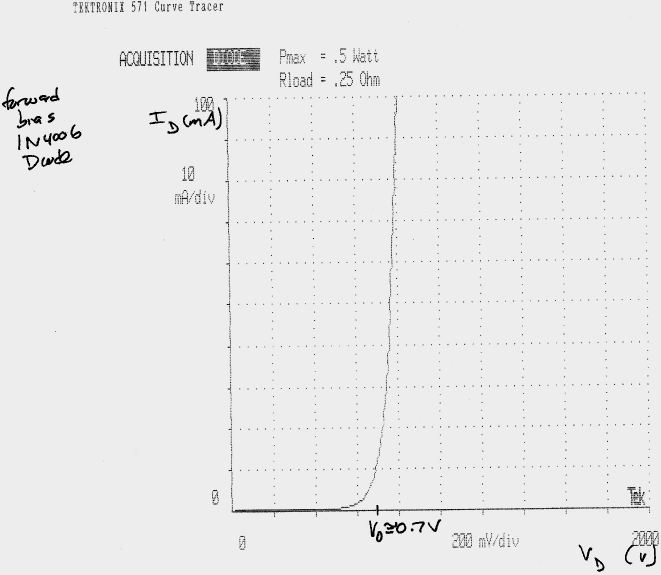
\includegraphics[width=4.25in]{img/diodeCurveTrace.png}
	\parbox{4.25in}{
	\caption{Curve tracer output for the~1N4006 silicon diode in a forward bias configuration.  Note that~$V_d=$\SI{0.7}{\volt}, as marked.}
	\label{fig:diodeCurve}}
\end{figure}

\begin{figure}[H]
	\centering
	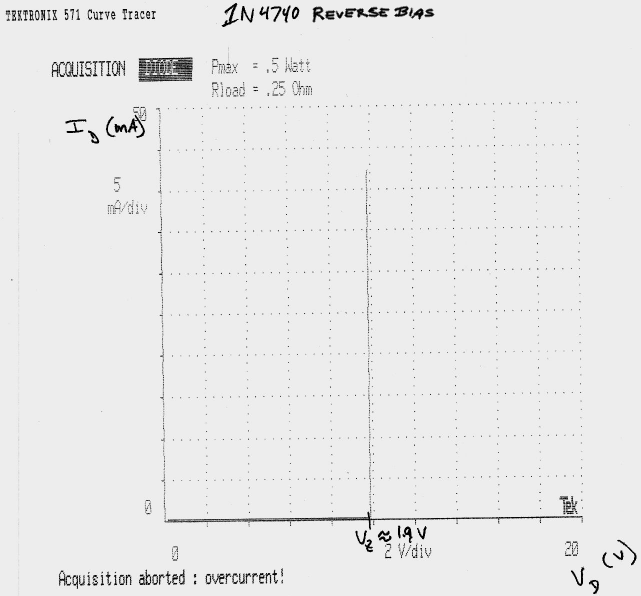
\includegraphics[width=4.25in]{img/zenerCurveTrace.png}
	\parbox{4.25in}{
	\caption{I-V curve for a~1N4740 zener diode in reverse bias.  The reverse
	breakdown voltage~$V_z$ is marked here as roughly~\SI{1.9}{\volt}.}
	\label{fig:zenerCurve}}
\end{figure}

\begin{figure}[H]
	\centering
	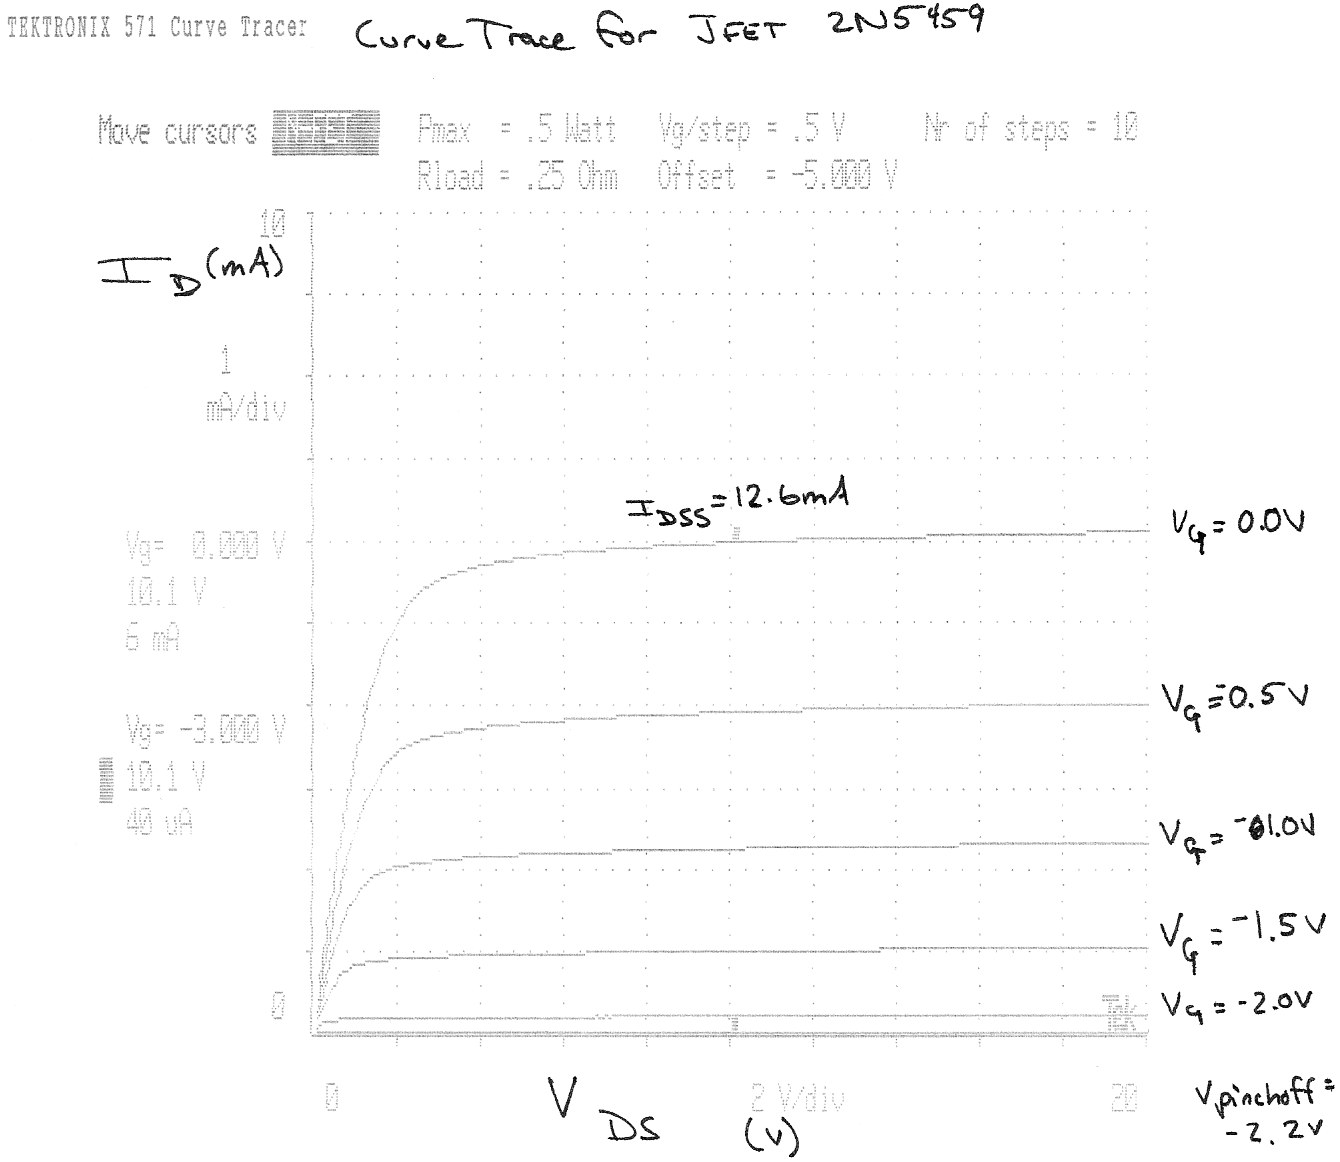
\includegraphics[width=4.25in]{img/jfetCurveTrace.png}
	\parbox{4.25in}{
	\caption{Traced I-V characteristics for a~2N5459 n-channel JFET.  Note the
	marked values of~$I_{DSS}$ (the current through the drain and source when the source is shorted to the gate) and~$V_{\text{pinchoff}}$
	as~\SI{12.6}{\milli\ampere} and~\SI{-2.2}{\volt}, respectively.}
	\label{fig:jfetCurve}}
\end{figure}



\section{License}
%Copyright \copyright\ 2011, Sean Barag.  All rights reserved.

Redistribution and use in source and binary forms, with or without
modification, are permitted provided that the following conditions are met:
\begin{itemize}
\item Redistributions of source code must retain the above copyright notice, this
  list of conditions and the following disclaimer.
\item Redistributions in binary form must reproduce the above copyright notice, this
  list of conditions and the following disclaimer in the documentation and/or
  other materials provided with the distribution.
\item Neither the name of the owner nor the names of its contributors may be
  used to endorse or promote products derived from this software without specific
  prior written permission.
\end{itemize}

THIS SOFTWARE IS PROVIDED BY THE COPYRIGHT HOLDERS AND CONTRIBUTORS ``AS IS'' AND
ANY EXPRESS OR IMPLIED WARRANTIES, INCLUDING, BUT NOT LIMITED TO, THE IMPLIED
WARRANTIES OF MERCHANTABILITY AND FITNESS FOR A PARTICULAR PURPOSE ARE
DISCLAIMED. IN NO EVENT SHALL THE COPYRIGHT HOLDER OR CONTRIBUTORS BE LIABLE
FOR ANY DIRECT, INDIRECT, INCIDENTAL, SPECIAL, EXEMPLARY, OR CONSEQUENTIAL
DAMAGES (INCLUDING, BUT NOT LIMITED TO, PROCUREMENT OF SUBSTITUTE GOODS OR
SERVICES; LOSS OF USE, DATA, OR PROFITS; OR BUSINESS INTERRUPTION) HOWEVER
CAUSED AND ON ANY THEORY OF LIABILITY, WHETHER IN CONTRACT, STRICT LIABILITY,
OR TORT (INCLUDING NEGLIGENCE OR OTHERWISE) ARISING IN ANY WAY OUT OF THE USE
OF THIS SOFTWARE, EVEN IF ADVISED OF THE POSSIBILITY OF SUCH DAMAGE.\\

Source code for this document is available at \texttt{http://github.com/sjbarag/}.


\end{document}
